\documentclass[10pt,a4paper]{article}
\usepackage[utf8]{inputenc}
\usepackage{amsmath}
\usepackage{amsfonts}
\usepackage{amssymb}
\usepackage{graphicx}
\usepackage{hyperref}
\usepackage[margin=1in]{geometry}
\usepackage{color}
\usepackage{algorithmicx}
\author{Jessica Chemali, Kumar Shaurya Shankar, Trenton Tabor\\ \{jchema,kumarsha,trent\}@cs.cmu.edu}
\title{16831 RoboStats Lab 2: \\Online Learning}
\begin{document}
\maketitle
\section{Overview}
\subsection{Discussion about Dataset}
The single biggest issue in the dataset is the bias in the data points. For instance the ground class and the vegetation class have two orders of magnitude data than, say the wires class. This disparity in the number of data points adversely affects linear classifier performance specially in a one-vs-all regime that we implement in this lab assignment. Thus, as shown later in the results, some classes are easily distinguishable but others like wire/pole are not. To mitigate this somewhat, we have tried to duplicate under-represented data in the training data. Further, since some of our algorithms are sensitive to the order in which training data is presented, we also shuffle the training data. We implemented k-fold cross validation to tune our parameters.
%----------------------------------------------------------------------
\section{Implemented methods}
\subsection{Bayes Linear Regression}
\subsubsection{Implementation}
The Bayes Linear Regressor has been implemented in Python, as is the rest of the framework. The external library dependency is only on numpy for matrix operations and normal distribution functions. We use scikit-learn for calculating the confusion matrix. The algorithm has not been modified for the purpose of this implementation.
\subsubsection{Parameter Selection}
The three parameter choices are the initial natural parameters for the prior on the weight vector, and the noise variance for the observation error. The latter was arbitrarily chosen, but {\color{blue}**TODO***} should be cross validated. For the prior, a 0 mean weight vector was chosen, and a hyper parameter of 1.0 for the precision matrix is chosen.

It was observed that because of the disparity in the class data for one vs all, and since mere duplication of under-represented data is not a good reflection of the actual distribution, we use margin scaling to assign a label of +10 to positive samples, and -1 to negative samples. This works fairly well in practice.
\subsubsection{Performance}
\begin{figure}[h]
\centering
\includegraphics[width=0.4\linewidth]{figs/BLR_3D_amtoan.png}
\includegraphics[width=0.4\linewidth]{figs/blr_amtoan.png}
\caption{Bayes Linear Regression trained on the am dataset, tested on the an dataset. The confusion matrix has been scaled column-wise to enhance visibility.}
\vspace{10pt}
\includegraphics[width=0.4\linewidth, trim = 0 0 0 35, clip]{figs/BLR_3D_antoam.png}
\includegraphics[width=0.4\linewidth]{figs/blr_antoam.png}
\caption{Bayes Linear Regression trained on the am dataset, tested on the an dataset. }
\label{}
\end{figure}
\begin{table}[h]
\centering
\begin{tabular}{|c|c|c||c|c|c|c|c||c||}
\hline
Comment&$\sigma$&$\Sigma_{prior}$&Veg & Wire & Pole & Ground & Facade & Accuracy\\ \hline
No noise&0.2 & 1.0 & 0.86951241 & 0.31436837 & 0.44126984 & 0.9800258 &  0.72926606 & 0.8518\\ \hline
+ 100 Random & 0.2 & 1.0 & 0.88313143 & 0.06222577 & 0.47450485 & 0.97512645 & 0.7285905  & 0.8557\\ \hline
$0.1 \sigma$ noise & 0.2 & 1.0 & 0.66242779 & 0.0436386  & 0.32891247 & 0.95459632 & 0.55975769 & 0.7186 \\ \hline
\end{tabular}
\caption{F1 score for BLR trained on am and tested on an}
\vspace{10pt}
\begin{tabular}{||c|c|c||c|c|c|c|c||c||}
\hline
Comment&$\sigma$&$\Sigma_{prior}$&Veg & Wire & Pole & Ground & Facade & Accuracy\\ \hline
No noise & 0.2 & 1.0& 0.87475848 & 0.35217954  &0.74221157  &0.99572913  &0.86710144 & 0.9554\\ \hline
+ 100 Random & 0.2 & 1.0 & 0.83830351 & 0.38423645  &0.68479117  &0.9956858  &0.86833179 &0.9538 \\ \hline
$0.1 \sigma$ noise & 0.2 & 1.0 & 0.583568 & 0.20260936 & 0.49171271 & 0.99528651  &0.45985532 & 0.8772\\ \hline
\end{tabular}
\caption{F1 score for BLR trained on an and tested on am}
\end{table}
\subsubsection{Learning Duration}
Training duration =  2.15570998192\\
Testing duration =  1.11386704445
\subsubsection{Robustness to Noise}
To test robustness we first added 100 uniform features to the feature vector. This resulted in a surprisingly negligible drop in performance
%------------------------------------------------------------------------
\subsection{Multiclass exponentiated gradient algorithm}

\subsubsection{Winnow with binary features}
We first implemented Winnow algorithm with binary features, after discretizing every feature based on the resulting entropy of the partition. It gave terrible results, because it turned out that the binary features weren't informative enough to differentiate well between the classes and the performance of the algorithm depended tremendously on the order the observations were presented to the algorithm. 

\subsubsection{Generalization of winnow to continuous features}

The algorithm that we will discuss is similar to winnow but instead, when the algorithm makes a mistake, it updates the weight of feature $i$ using the equation : $w_i = w_i*exp(\nu x_i y_i)$. 

Training online was affected considerably by the order the data was presented to the algorithm. This is why we shuffled the data before training the algorithm and in this way reached better results.

Training on the "an" dataset and testing on the held out "am" dataset was easier than the other way around and resulted in an accuracy of around $90\%$ versus an accuracy of $70\%$ on the held out datasets. The confusion matrix, which is more useful showed that the algorithm predicted very well class $1200$ with very little negatives, followed by class $1004$, and class $1400$. Classes $1100$ and $1103$, corresponding to the poles and wires were poorly learned. This is not surprising because the datasets were highly unbalanced and relatively very few observations were from a pole or a wire. Although we tried to balance the number of observations from each class, the configuration of the features observed were still limited.

The implementation of the algorithm is straightforward, it is only a few lines of code in python. We train binary learners for each of the class and combine them for multi-class classification. The algorithm is very fast. For learning it loops through the $n$ observations and at each step it updates the weights of all $d$ features. We learn $c$ classifiers. The computational complexity of learning is therefore $O(n*d*c)$. For prediction, a dot product is taken for each of the classes and the best one is selected, so the computational complexity is $O(d*c)$

For this algorithm we had 2 hyperparameters to tune: the learning rate $\nu$, and a threshold $\theta$. We looked at $\nu = \{0.001,0.01,0.1\} \times \theta = \{5,10,15\}$ and compared them against each other using 5-fold cross validation. the results were obtained with $\nu = 0.01$ and $\theta = 10$.

{\color{blue} PLEASE ADD RESUlTS FROM noisy features for winnow. thanks you!}
\begin{figure}[htp]
\centering
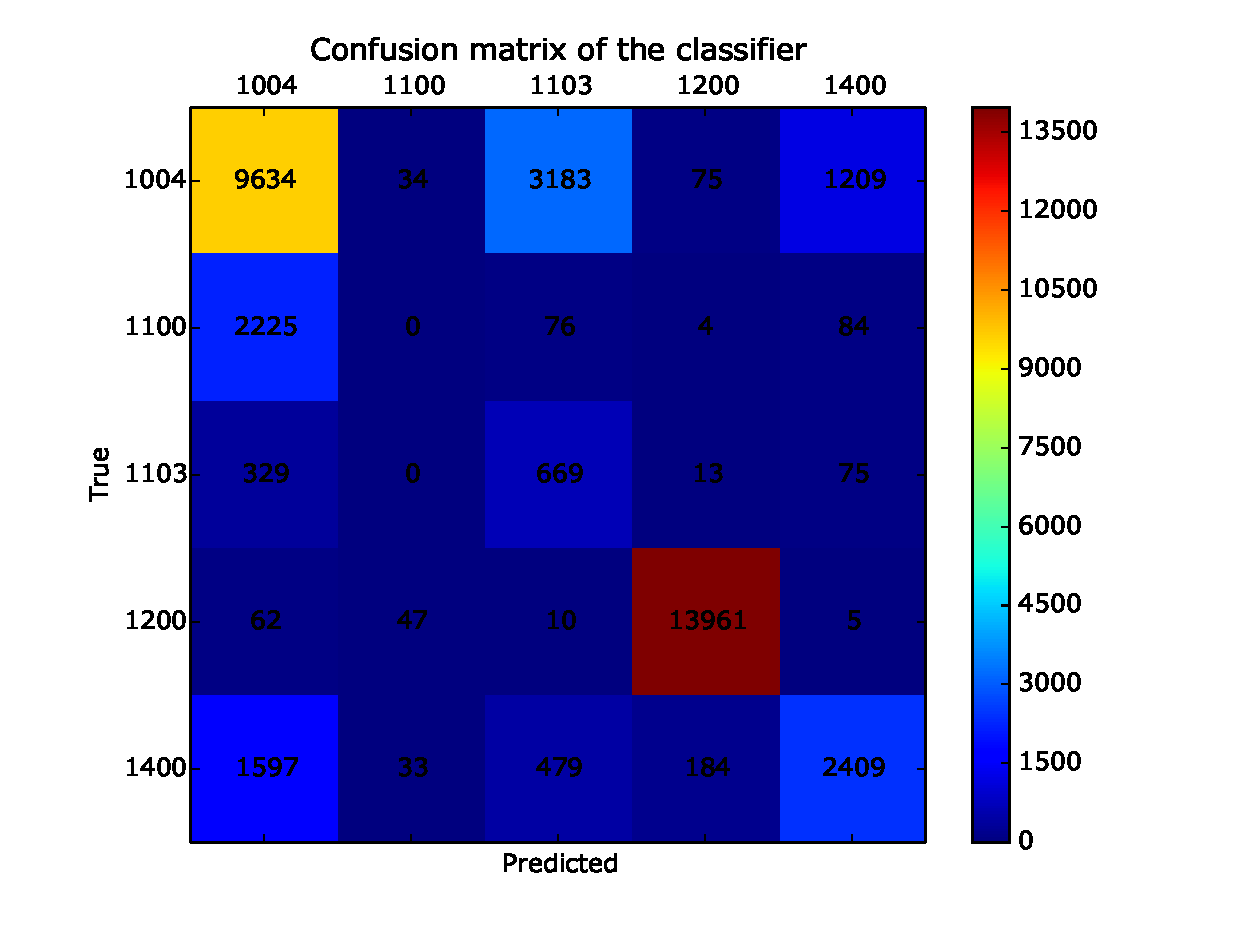
\includegraphics[scale=0.4,trim = 0.3 0.3 0.3 0.3,clip]{figs/winnow_amtoan_test1.eps}
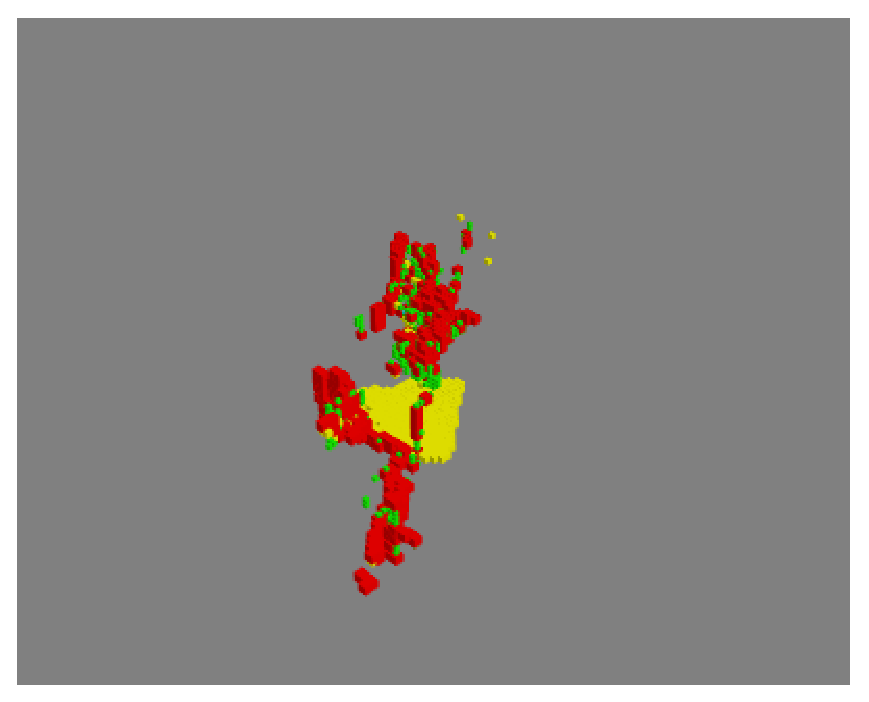
\includegraphics[scale=0.4]{figs/winnow_amtoan_test1_plot.eps}
\caption{Multiclass Winnow trained on the am dataset, testing on the an}
\vspace{0.1 in}
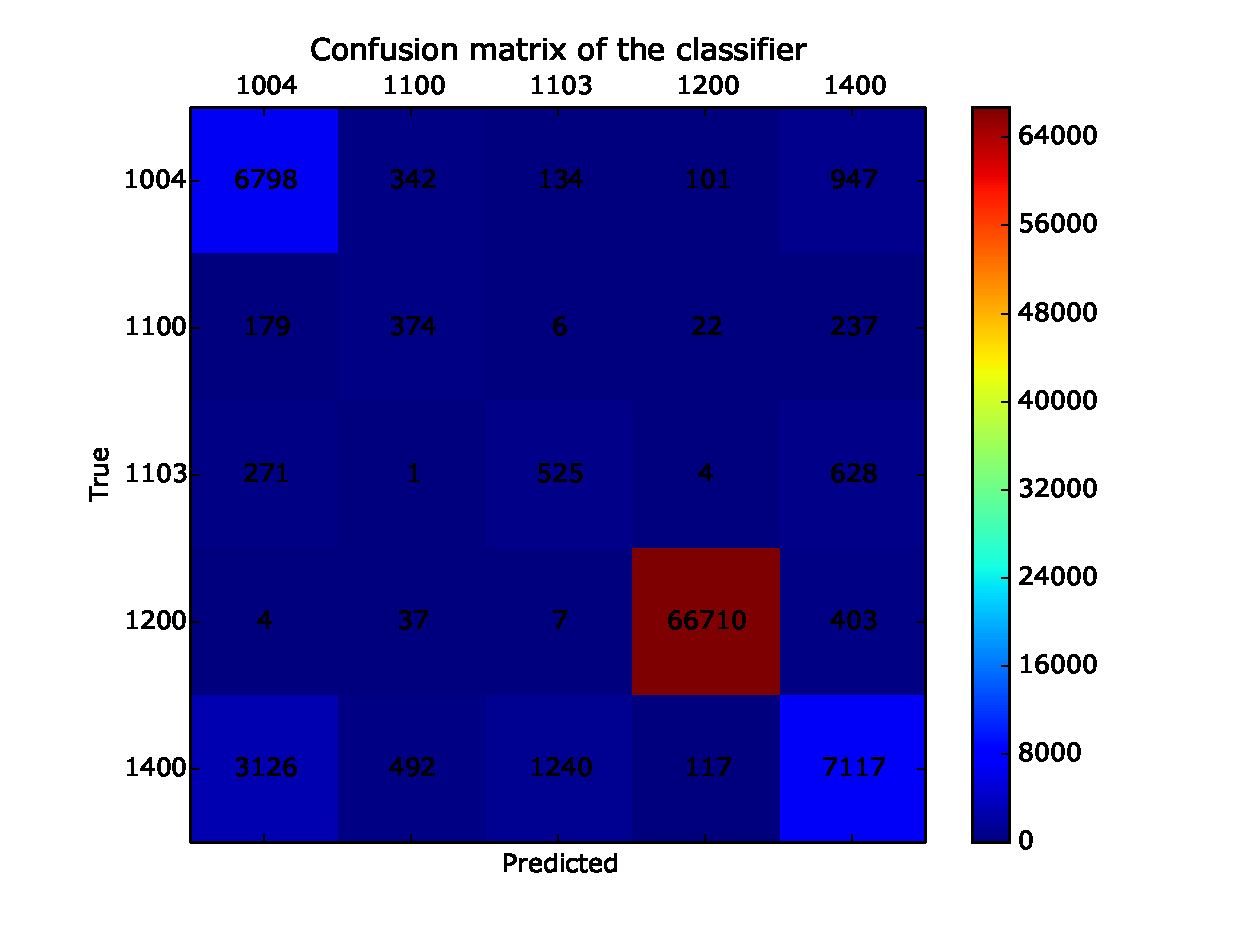
\includegraphics[scale=0.4,trim = 0.3 0.3 0.3 0.3,clip]{figs/winnow_antoam_test1.eps}
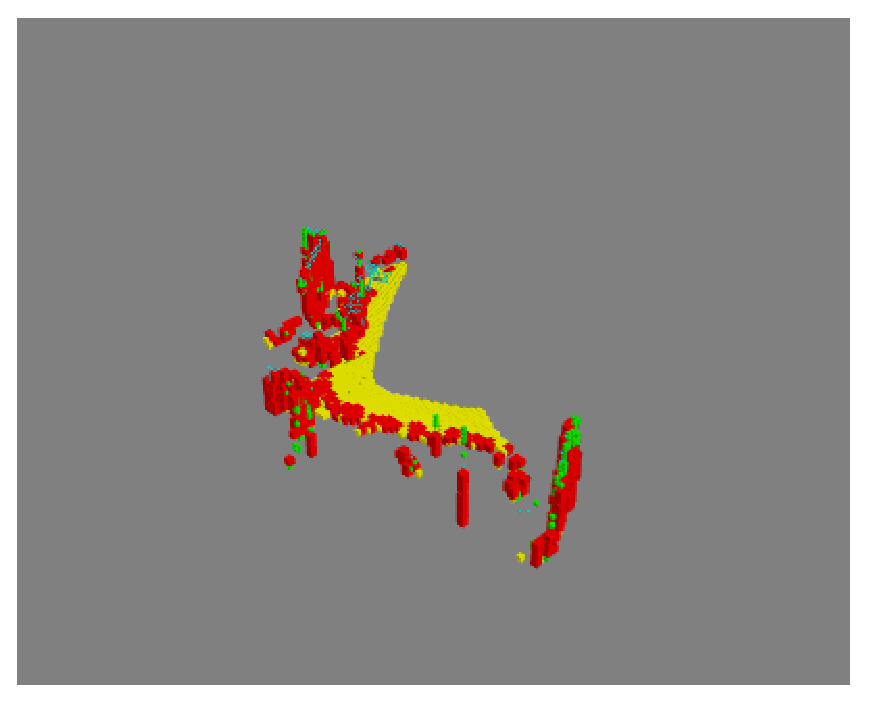
\includegraphics[scale=0.4]{figs/winnow_antoam_test1_plot.eps}
\caption{Multiclass Winnow trained on the an dataset, testing on the am}
\label{}
\end{figure}


%----------------------------------------------------------------------
\subsection{Kernalized SVM}
\subsubsection{Implementation}
We use the algorithm discussed in class for implementation. Specific modifications that we make are to not compute the regularizer term of the loss function for performance reasons. We do this since estimating the $\langle f, f \rangle = \alpha^T K_{ij} \alpha$ is an expensive operation. The update step, however, uses the standard regularizer term for shrinking $\alpha$s at each step. The kernel we choose is a simple dot product kernel, i.e. $k(x_i, x_j) = x_i^T x_j$. In order for the support vectors to not fill up memory and slow down the training, we choose to drop support vectors for which the magnitude of $\alpha$ falls below $1e-10$

For each trained one vs all predictor we add positive samples till a certain proportion ($0.2$) of the rest of the data points. We then assign these positive samples a label of +1 and all the negative samples a label of -1
\subsubsection{Parameter Selection}
The two main parameters for our dot product kernel are the learning rate and the regularizer. The smaller the learning rate, the larger the number of support vectors are added, and the more representative the overall function is. The regularizer term effectively controls the shrinking of the $\alpha$s. 

\subsubsection{Performance}
\begin{figure}[h]
\centering
\includegraphics[width=0.4\linewidth]{figs/BLR_3D_amtoan.png}
\includegraphics[width=0.4\linewidth]{figs/blr_amtoan.png}
\caption{Bayes Linear Regression trained on the am dataset, tested on the an dataset. The confusion matrix has been scaled column-wise to enhance visibility.}
\vspace{10pt}
\includegraphics[width=0.4\linewidth, trim = 0 0 0 35, clip]{figs/BLR_3D_antoam.png}
\includegraphics[width=0.4\linewidth]{figs/blr_antoam.png}
\caption{Bayes Linear Regression trained on the am dataset, tested on the an dataset. }
\label{}
\end{figure}
%-----------------------------------------------------------------------
\section{Comparative Analysis of Learners}
SVM fits the best to the data due to the advantage of the kernels.

\section{Future Work}
Augment features using spatial context, e.g., 3D HoG.\\
\end{document}